\documentclass[journal ]{new-aiaa}
%\documentclass[conf]{new-aiaa} for conference papers
\usepackage[utf8]{inputenc}
\usepackage{textcomp}

\usepackage{graphicx}
\usepackage{amsmath}
\usepackage[version=4]{mhchem}
\usepackage{siunitx}
\usepackage{longtable,tabularx}
\setlength\LTleft{0pt} 

\title{A Comprehensive Review on the Development of Computational Frameworks for Spacecraft Fragmentation and Orbital Debris Population Dynamics}

\author{Juan F Puerta \footnote{Insert Job Title, Department Name, Address/Mail Stop, and AIAA Member Grade (if any) for first author.}}
\affil{Business or Academic Affiliation 1, City, State, Zip Code}
\author{Nicolás Muñoz-Galeano\footnote{Research Group in Efficient Energy Management (GIMEL), Departamento de Ingeniería Eléctrica, Universidad de Antioquia, Calle 67 No. 56-108, Medellin 050010, Colombia;nicolas.munoz@udea.edu
(N.M.-G.)}}
\affil{Business or Academic Affiliation 1, City, State, Zip Code}

\author{Third C. Author\footnote{Insert Job Title, Department Name, Address/Mail Stop, and AIAA Member Grade (if any) for third author.}}


\begin{document}

\maketitle

\begin{abstract}
These instructions give you guidelines for preparing papers for AIAA Technical Journals using \LaTeX{}. If you previously prepared an AIAA Conference Paper using the Meetings Papers Template, you may submit using the Meetings Papers Template so long as the text is double-spaced.  Carefully follow the journal paper submission process in Sec.~II of this document. Keep in mind that the electronic file you submit will be formatted further at AIAA. This first paragraph is formatted in the abstract style. Abstracts are required for regular, full-length papers and express articles. Be sure to define all symbols used in the abstract, and do not cite references in this section. The footnote on the first page should list the Job Title and AIAA Member Grade (if applicable) for each author.
\end{abstract}

\section*{Nomenclature}

\noindent(Nomenclature entries should have the units identified)

{\renewcommand\arraystretch{1.0}
\noindent\begin{longtable*}{@{}l @{\quad=\quad} l@{}}
$A$  & amplitude of oscillation \\
$a$ &    cylinder diameter \\
$C_p$& pressure coefficient \\
$Cx$ & force coefficient in the \textit{x} direction \\
$Cy$ & force coefficient in the \textit{y} direction \\
c   & chord \\
d$t$ & time step \\
$Fx$ & $X$ component of the resultant pressure force acting on the vehicle \\
$Fy$ & $Y$ component of the resultant pressure force acting on the vehicle \\
$f, g$   & generic functions \\
$h$  & height \\
$i$  & time index during navigation \\
$j$  & waypoint index \\
$K$  & trailing-edge (TE) nondimensional angular deflection rate\\
$\Theta$ & boundary-layer momentum thickness\\
$\rho$ & density\\
\multicolumn{2}{@{}l}{Subscripts}\\
cg & center of gravity\\
$G$ & generator body\\
iso	& waypoint index
\end{longtable*}}




\section{Introduction}
\lettrine{I}{n} this section, you will briefly introduce the context of the PhD research will be introduced to highlight the relevance of conducting a bibliometric analysis. Here is what to include:

\begin{itemize}
    \item Research Context: Give a brief overview of your research topic in aerospace engineering. For example, if you are working on space debris mitigation, describe why this field is critical to aerospace engineering.
    \item Rationale for Bibliometric Analysis: Explain why bibliometrics are useful for identifying trends, influential publications, and key authors in your research area. Emphasize how tools like VOSviewer and pybibx can help map the academic landscape.
    \item Purpose and Objectives: Clearly state the purpose of the review and what you aim to uncover through your bibliometric analysis (e.g., gaps in the literature, influential papers, emerging themes).
\end{itemize}

\section{Methodology}

To provide a comprehensive review of spacecraft fragmentation and orbital debris, a multistage search strategy using several databases such as Scopus and Google Scholar  was developed. Scopus, which is one of the largest abstract and citation databases for peer-reviewed literature, was selected intensively for its extensive coverage of the aerospace and engineering domains. A series of four targeted searches were conducted, each focusing on a specific aspect related to orbital debris and spacecraft fragmentation, as well as relevant computational methods for orbital analysis.

These queries were: “spacecraft fragmentation orbital debris,” “space debris orbit propagator,” “symplectic orbit integrators,” and “n-body REBOUND.” Each search query addressed a specific subtopic of interest within the broader theme of spacecraft fragmentation and orbital debris dynamics.

\begin{itemize}
    \item Spacecraft Fragmentation Orbital Debris: This search focused on identifying literature that discusses the mechanisms and consequences of spacecraft fragmentation and the subsequent creation of orbital debris. The goal was to gather insights into the formation, characteristics, and hazards of debris generated through fragmentation events. 149 papers were found.
    \item Space Debris Orbit Propagator: The second query aimed to retrieve papers related to the modeling and simulation of orbital debris trajectories, specifically focusing on orbit propagators that predict the movement of debris over time. This is critical for understanding how debris evolves in Earth’s orbit and poses risks to operational spacecraft. 101 papers were found.
    \item Symplectic Orbit Integrators: This search was designed to identify papers that examine the use of symplectic integration methods for long-term orbit propagation. Symplectic integrators are known for their ability to maintain the stability of orbit calculations over extended periods, making them essential in debris modeling and collision risk assessments. 183 papers were found.
    \item N-body REBOUND: The fourth query focused on the use of n-body simulation techniques and the REBOUND code to model the interactions between multiple objects in space. This technique is particularly useful for analyzing complex interactions within orbital debris clouds and assessing potential collision scenarios. 31 papers were found.
\end{itemize}

A combination of these four search queries ensured that the resulting set of papers covered both theoretical and practical aspects of spacecraft fragmentation, orbital debris dynamics, and advanced simulation methods. After conducting the searches, a total of xx papers were identified as relevant and selected for further analysis. The inclusion criteria for the articles were based on their relevance to the topic, publication in peer-reviewed journals or conferences, and availability of full-text access. Papers older than 20 years or those with minimal citations were excluded unless they contributed to foundational theories or models still referenced today.

\subsection{VOSviewer and PyBibX Analysis}
To analyze the selected articles and identify key trends, the VOSviewer and PyBibX tools were used. VOSviewer is a widely-used software tool designed for creating and visualizing bibliometric networks. It is especially useful in generating network maps based on data from bibliographic databases such as Scopus and Web of Science. These networks can represent relationships between various entities, including co-authorship networks, citation networks, keyword co-occurrence networks, and bibliographic coupling.VOSviewer was used to perform bibliometric analyses such as citation mapping, co-occurrence keyword networks, and bibliographic coupling of organizations. This allowed for visualization of relationships between papers, keywords, and contributing institutions, providing insights into the most influential authors and trends in the field.

In addition, PyBibX is a Python-based tool that is used for advanced bibliometric analysis. While VOSviewer specializes in visualization, PyBibX focuses more on providing detailed bibliometric metrics and analysis of citation data. It can be used to extract and analyze bibliometric data from sources like Scopus and Web of Science as well, and it allows for flexible, customized analysis using Python.

The citation analysis revealed the most frequently cited papers, highlighting seminal works that have shaped the current understanding of spacecraft fragmentation and orbital debris. Keyword co-occurrence analysis enabled the identification of the most prominent research themes, including orbital debris mitigation, collision risk assessment, and debris propagation modeling. Additionally, bibliographic coupling allowed for the identification of key institutions, such as NASA, the European Space Agency (ESA), and leading universities that have contributed extensively to the body of knowledge on orbital debris.

Through this combination of Scopus searches and advanced bibliometric tools, the review was able to provide a detailed synthesis of the current state of research and identify areas where further investigation is needed.

\section{Analysis Results}

Core findings of the bibliometric analysis:

Based on the methodology described in the last section, these are the results.

\subsection{Spacecraft fragmentation orbital debris}

\subsubsection{Author Citation}

\begin{figure}[hbt!]
\centering
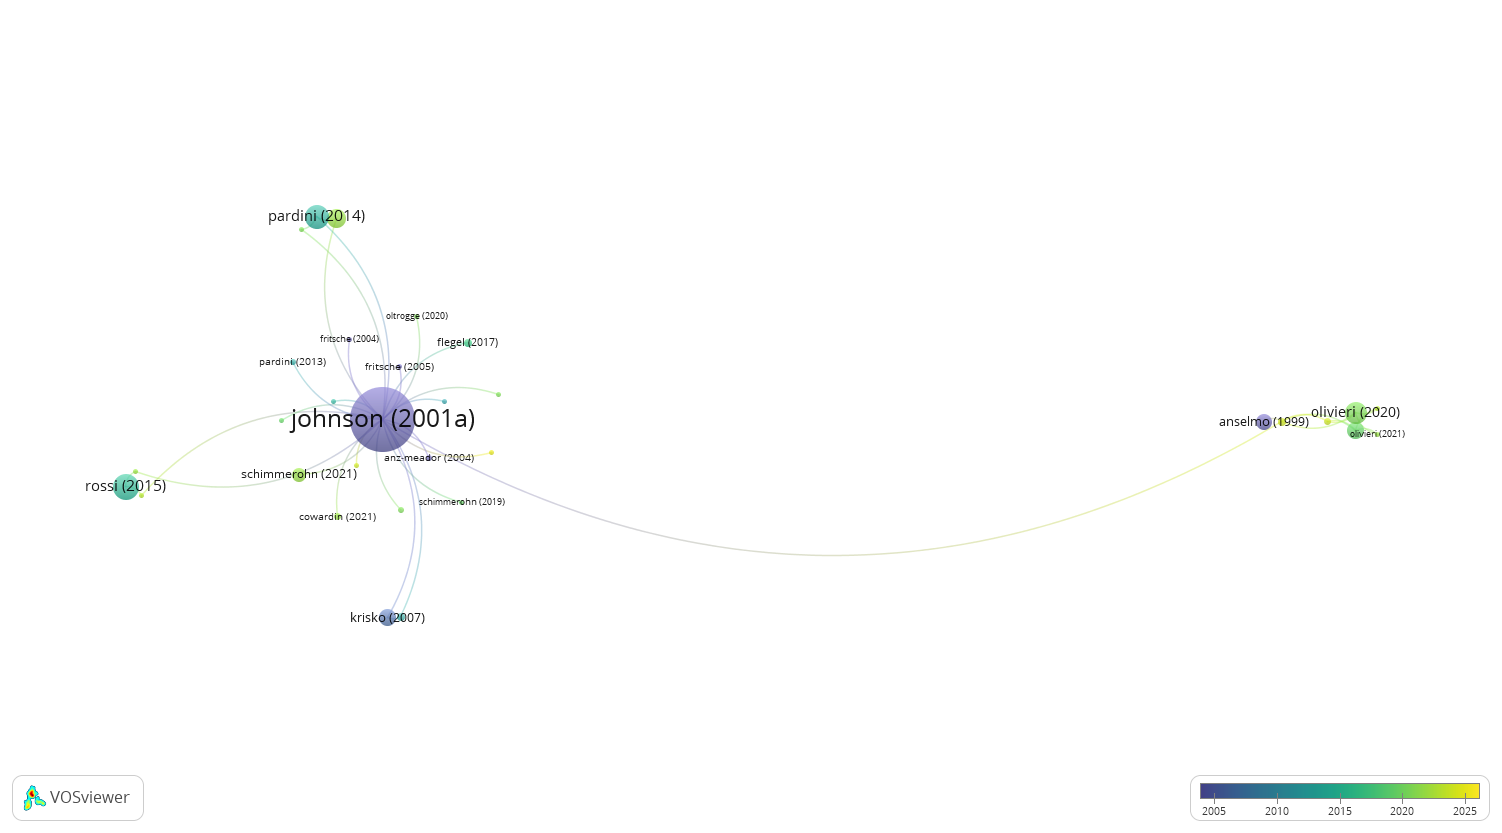
\includegraphics[width=\textwidth]{sfod_citation.png}
\caption{Spacecraft fragmentation orbital debris author citation in VosViewer.}
\end{figure}

This image is a visualization of the citation network generated by VOSviewer, based on a bibliometric analysis of papers related to spacecraft fragmentation and orbital debris, using the data extracted from Scopus. The image provides several insights based on the relationships between papers and the way they cite each other. Each circle represents a paper, and the size of each node indicates its relevance or importance in the network based on the number of citations it has received. A larger node means a paper that has been cited frequently in other works. The lines connecting the nodes represent the citation links between the papers. The more connected a node is, the more it has influenced other works in the domain.

\textbf{Clusters and Groups.}

\begin{itemize}
    \item Johnson (2001a) is clearly a central and highly influential paper in this field. Its central position and large node size indicate that many subsequent works refer to it. Several other papers, such as Krisko (2007) and Pardini (2014), are clustered around Johnson's work, suggesting that they are closely related or have built upon its findings.
    \item Rossi (2015) and Olivieri (2020) are also notable, although somewhat isolated compared to Johnson's paper, but still showing relevance in the field.
    \item The connection between Johnson (2001a) and Krisko (2007) likely suggests that these papers are foundational in the field of spacecraft fragmentation and orbital debris, and they have provided significant contributions that are built upon by others.
\end{itemize}

\textbf{Color Gradient (Timeline).}

\begin{itemize}
    \item The coloring of the nodes represents the publication timeline of these works. Papers in blue and purple are from earlier years (likely 1999-2005), while yellow and green represent newer papers published in more recent years (closer to 2020-2025).
    \item Johnson (2001a) is an older but highly cited work, which has spawned numerous follow-up studies over the years, indicated by connections to papers in green and yellow.
    \item Olivieri (2020) and its connected papers in green and yellow highlight recent developments in the domain of space debris fragmentation, indicating active research interest.
\end{itemize}

\textbf{Notable Connections.}

\begin{itemize}
    \item The presence of Rossi (2015) and its connection to the network indicates a significant contribution, though it may be on a different subtopic compared to the core cluster around Johnson (2001a).
    \item The network on the right, around Olivieri (2020), suggests newer and potentially more innovative research trends, especially in 2020 and beyond, signaling emerging research areas in the field.
\end{itemize}

\textbf{Analysis.}
\begin{itemize}
    \item Johnson (2001a) remains a seminal work in spacecraft fragmentation and orbital debris, influencing multiple subsequent papers and studies. It likely presents foundational theories, models, or data that have shaped much of the current understanding in the field.
    \item Rossi (2015) and Olivieri (2020) represent important contributions, particularly in more recent developments. However, they appear slightly isolated, suggesting that these papers might be focusing on different or novel approaches that are less directly connected to the foundational models of the earlier papers.
    \item The density of connections between nodes, particularly around Johnson (2001a), indicates that much of the research on space debris fragmentation is interrelated, with researchers building upon previous works to expand the body of knowledge.
    \item The timeline of publications shows that research in this field is ongoing, with new insights and models being published through 2020-2025, indicating that the problem of orbital debris is an active and evolving area of study.
\end{itemize}

\subsubsection{Co-occurrence keywords.}

\begin{figure}[hbt!]
\centering
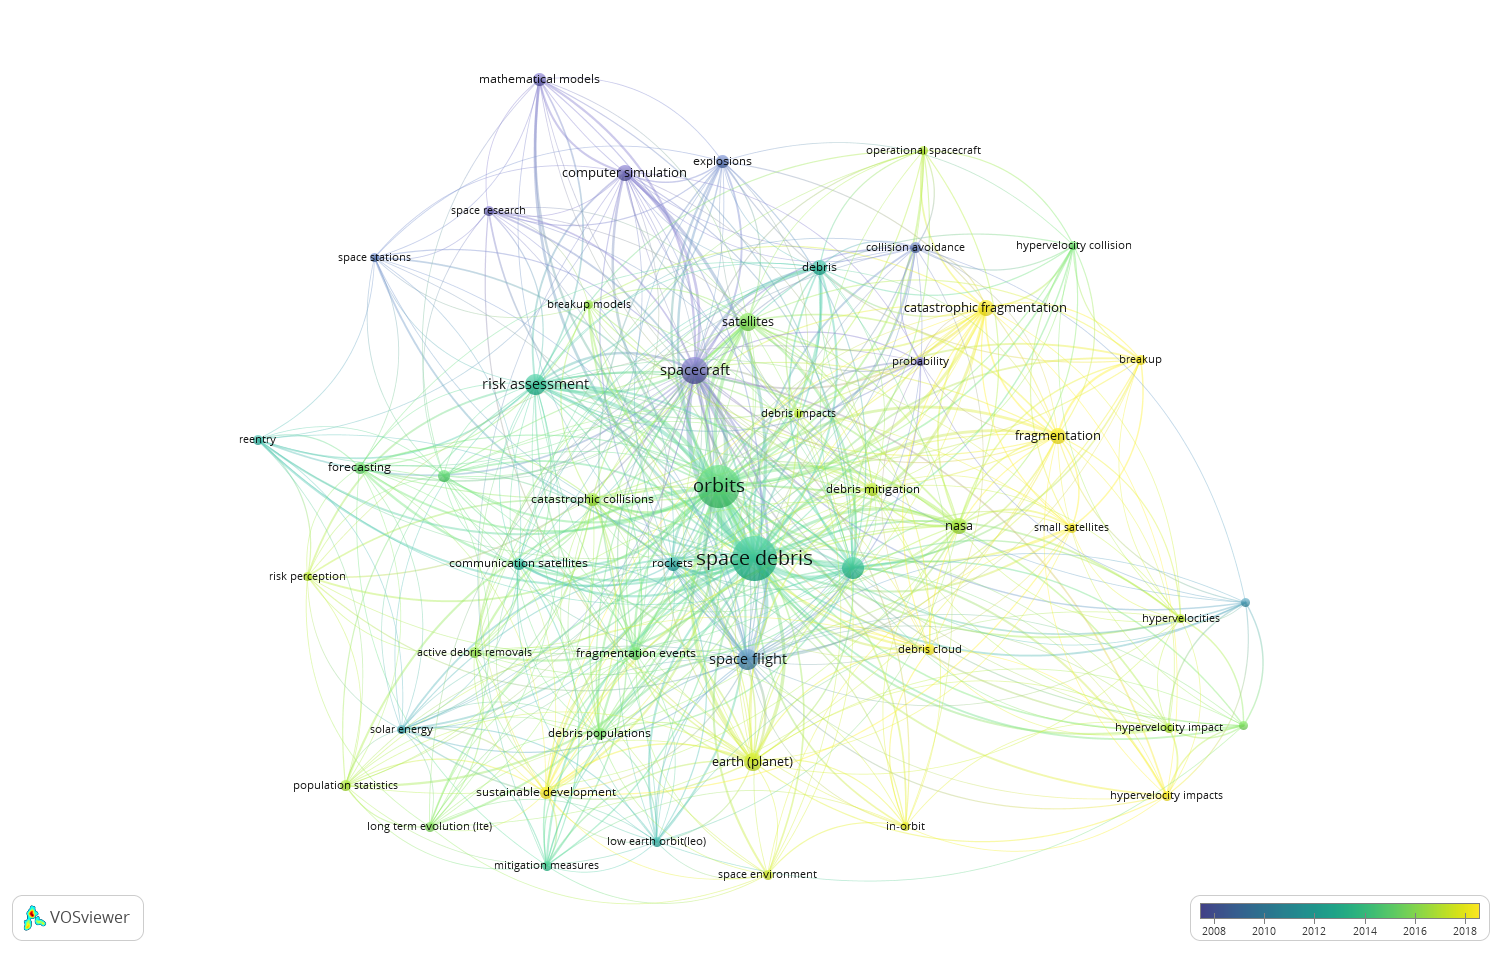
\includegraphics[width=\textwidth]{sfod_coocurrence_keywords.png}
\caption{Spacecraft fragmentation orbital debris keyword co-occurrence in VosViewer.}
\end{figure}

This image represents a co-occurrence network of keywords related to spacecraft fragmentation and orbital debris, based on the bibliometric analysis of publications from Scopus. Each node represents a keyword, and the connections between them show how frequently these keywords appear together in academic papers.

\textbf{Central Cluster (green/yellow).}

\begin{itemize}
    \item Core keywords include "space debris", "orbits", and "space flight". These keywords are at the heart of the research and are highly related to a wide range of other topics.
    \item The focus on space debris indicates that this is the primary issue being addressed in this research area. The term is connected to several adjacent topics like debris mitigation, fragmentation, debris clouds, and operational spacecraft.
    \item NASA appears prominently, suggesting a strong involvement of the agency in both research and mitigation efforts related to space debris.
\end{itemize}

\textbf{Top-Left Cluster (purple/blue).}

\begin{itemize}
    \item This cluster includes keywords such as "mathematical models", "computer simulation", and "space research".
    \item These terms are older and focus on the modeling and simulation aspects of space debris and fragmentation, which form the basis for theoretical understanding.
    \item Mathematical models are critical for simulating the behavior of space debris and predicting collision risks, forming the backbone of fragmentation analysis and orbital debris studies.
\end{itemize}

\textbf{Right Side Cluster (green/yellow).}

\begin{itemize}
    \item This cluster focuses on more technical and operational aspects of fragmentation, including terms such as "fragmentation", "catastrophic fragmentation", and "hypervelocity impacts".
    \item This suggests a more recent interest in high-speed collisions and the effects of hypervelocity on debris, which are important in understanding how fragmentation events generate more debris in space.
    \item The terms breakup and catastrophic fragmentation indicate that research has shifted toward studying the severe consequences of fragmentation events and their impact on space missions.
\end{itemize}

\textbf{Bottom Cluster (green/yellow).}

\begin{itemize}
    \item Keywords such as "sustainable development", "low earth orbit" (LEO), "mitigation measures", and "active debris removal" show the growing importance of sustainability in space operations.
    \item The emphasis on mitigation suggests that researchers are focusing on solutions to the space debris problem, such as debris removal technologies and disposal strategies.
    \item Low Earth Orbit (LEO) is of particular concern because it is a densely populated orbital region, and many mitigation efforts focus on keeping this region clear of hazardous debris.
\end{itemize}

\textbf{Top-Right Cluster (yellow/green).}

\begin{itemize}
    \item This small, more recent cluster revolves around specific topics like "hypervelocity collisions", "debris impacts", and "collision avoidance".
    \item These topics are critical for modern-day spacecraft operations, as the risk of collisions with debris is one of the main operational challenges in space.
\end{itemize}

\subsubsection{Coupling organizations.}

\begin{figure}[hbt!]
\centering
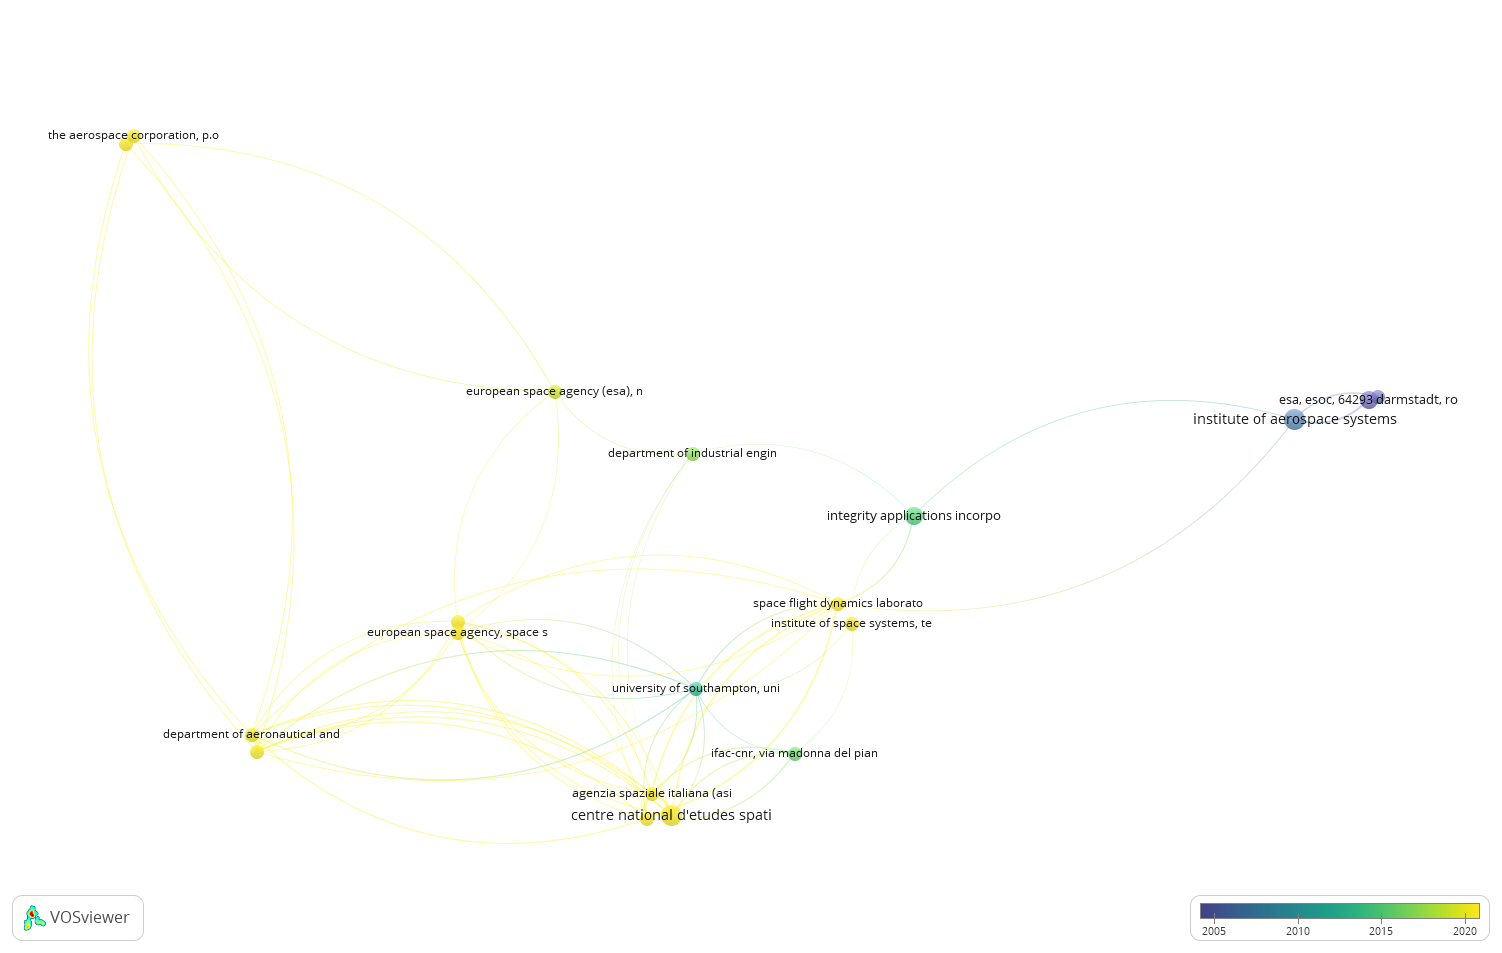
\includegraphics[width=\textwidth]{sfod_b-coupling_organizations.png}
\caption{Spacecraft fragmentation orbital debris coupling organizations reference in VosViewer.}
\end{figure}

 This visualization represents bibliographic coupling of organizations in the field of spacecraft fragmentation and orbital debris. Bibliographic coupling occurs when two organizations cite the same third-party paper, indicating that they are likely researching similar topics.

\textbf{Left Side (Yellow/Green Cluster).}

\begin{itemize}
    \item Organizations like The Aerospace Corporation and European Space Agency (ESA) dominate this side of the graph.
    \item The ESA appears multiple times, which likely indicates that its sub-organizations (e.g., European Space Agency, Space S, European Space Agency (ESA), etc.) are actively collaborating or working on distinct but related projects.
    \item This cluster focuses on more recent research (yellow nodes), with strong involvement from space agencies such as ESA and Agenzia Spaziale Italiana (ASI). These agencies are at the forefront of recent developments in spacecraft fragmentation and debris management.
\end{itemize}

\textbf{Right Side (Blue/Green Cluster).}

\begin{itemize}
    \item ESA's European Space Operations Centre (ESOC) of ESA in Darmstadt, together with the Institute of Aerospace Systems, form an important node in this region. These organizations are linked with more historical research (blue nodes), and are still relevant but with less recent output compared to the yellow cluster.
    \item ESOC seems to be a key player in early works on spacecraft fragmentation and orbital debris, likely focusing on space operations and debris monitoring.
\end{itemize}

\textbf{Middle Cluster (Mixed Timeline).}

\begin{itemize}
    \item University of Southampton, Space Flight Dynamics Laboratory, IFAC-CNR, and other institutions make up this middle ground, with green nodes. These institutions have more balanced contributions over time.
    \item University of Southampton and other academic institutions appear to play a bridging role between highly specialized space agencies and technical laboratories, as they collaborate with both.
\end{itemize}

\textbf{Analysis.}
\begin{itemize}
    \item Core Institutions: The European Space Agency (ESA) is a central node, with many of its sub-organizations actively involved in research related to space debris. Aerospace Corporation and European institutions like CNES (Centre National d'Études Spatiales) and ASI are also key players. Their strong coupling indicates that these institutions are leading the charge in studying spacecraft fragmentation and mitigating orbital debris.
    \item Recent and Historical Contributions.
    \begin{itemize}
        \item Organizations with yellow nodes represent more recent contributors to the research, including ESA and its associated projects.
        \item Blue and green nodes represent historically significant contributors, like ESOC, who have been publishing since earlier years but are still relevant.
    \end{itemize}
    \item Space Agencies and Academia: There seems to be a strong collaboration between space agencies (ESA, ASI, CNES) and academic institutions (University of Southampton, Institute of Aerospace Systems), suggesting a synergistic relationship where space missions and practical operations are informed by academic research and vice versa.
\end{itemize}

\textbf{Insights and Implications.}
\begin{itemize}
    \item ESA's Role: The prominence of ESA and its multiple sub-organizations indicates its leadership in space debris management research. Their coupling with other institutions suggests that they are working closely with both European and international partners.
    \item Inter-agency and Inter-institutional Collaboration: The network highlights inter-agency cooperation, as seen between ESA, Aerospace Corporation, CNES, and ASI. Such collaboration is vital for addressing global challenges such as space debris.
    \item Shifting Focus Over Time: The color gradient suggests a transition in the focus of research. Earlier work (blue nodes) might have laid the theoretical foundations, while more recent publications (yellow nodes) likely focus on applied solutions and mitigation techniques.
    \item Geographical Diversity: The institutions in this network span different countries, indicating the international nature of space debris research. This is a field that benefits from global cooperation, as space debris affects all nations with space programs.
\end{itemize}


\begin{figure}[hbt!]
\centering
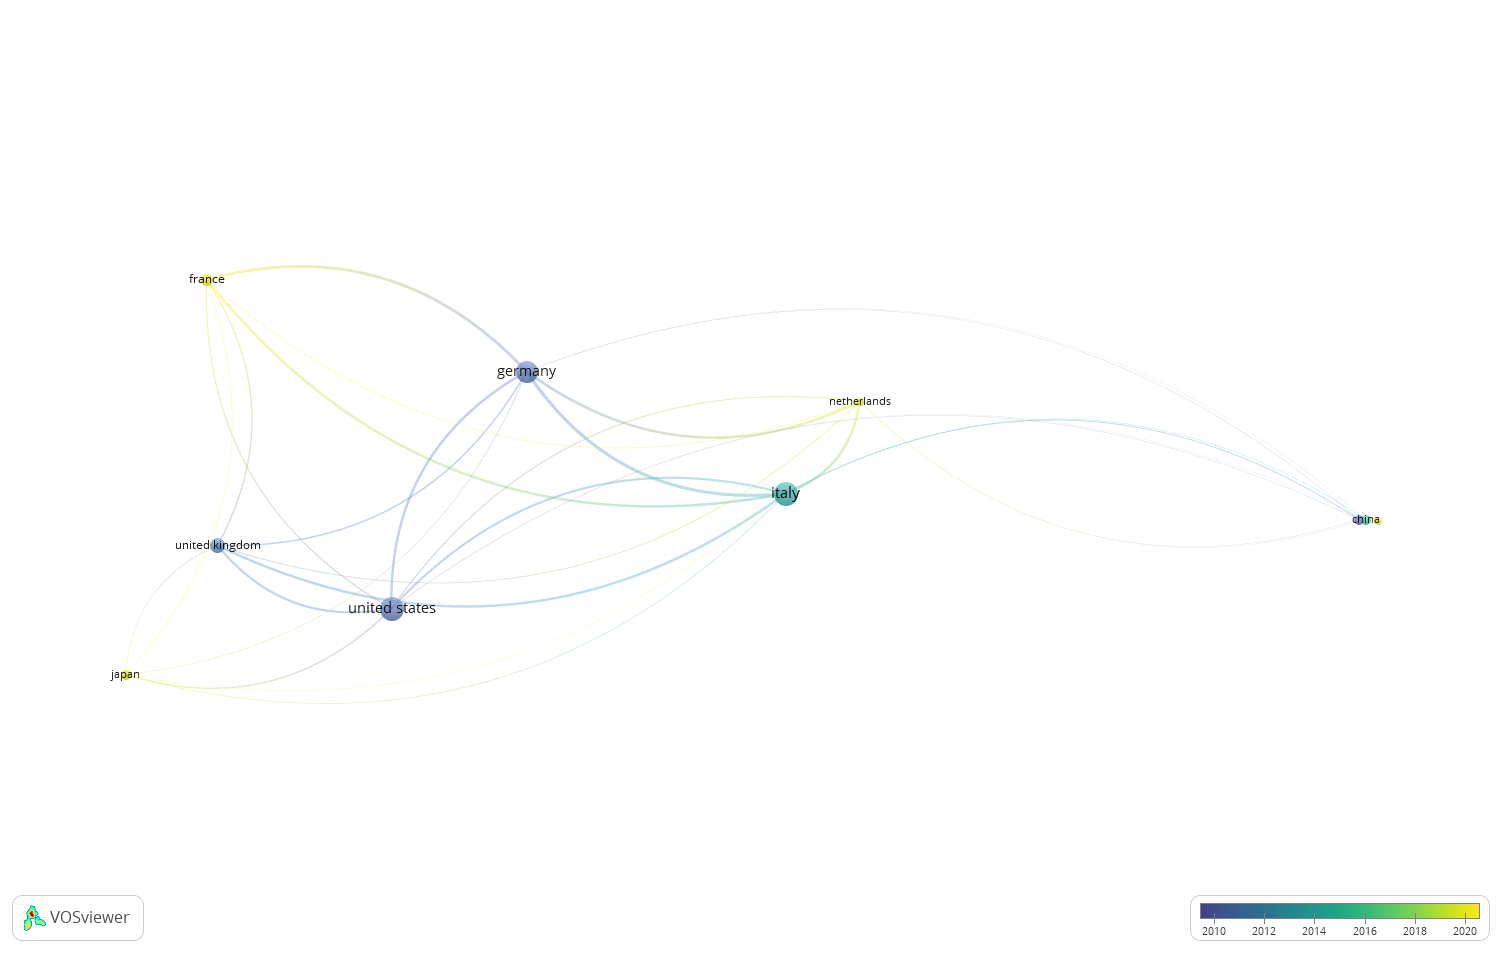
\includegraphics[width=\textwidth]{sfod_b-coupling_countries.png}
\caption{Spacecraft fragmentation orbital debris coupling countries citation in VosViewer.}
\end{figure}





\begin{itemize}
    \item Descriptive Statistics: Start by presenting basic descriptive data from Scopus, such as:
    \begin{itemize}
        \item Number of papers, authors, journals, and citations.
        \item Trends over time (e.g., increase in publications per year).
        \item Top journals publishing in aerospace engineering.
        \item Leading countries and institutions.
    \end{itemize}
    \item Co-Authorship Networks (using VOSviewer):
    \begin{itemize}
        \item Present a co-authorship network map, showing the collaboration patterns between authors, institutions, or countries.
        \item Discuss key authors and institutions with high centrality in the network and their impact on the field.
    \end{itemize}
    \item Keyword Co-occurrence Networks (using VOSviewer):
    \begin{itemize}
        \item Present keyword co-occurrence maps to reveal the main themes, trends, and topics in aerospace engineering research.
        \item Highlight key research topics and clusters.
    \end{itemize}
    \item Citation Analysis:
    \begin{itemize}
        \item Analyze and visualize the citation patterns to identify influential papers, journals, and authors.
        \item Discuss how certain works have shaped the research field.
    \end{itemize}
    \item Emerging Topics and Trends:
    \begin{itemize}
        \item Use the co-word analysis to identify emerging topics or gaps in the research (e.g., growing focus on reusable launch systems, satellite collision avoidance).
    \end{itemize}
\end{itemize}

\section{Discussion}

Interpret the results of the bibliometric analysis, comparing them with the existing state of the literature. Discuss the following.

\begin{itemize}
    \item Key Authors and Influential Publications: Who are the thought leaders? Which papers are highly cited? How do they contribute to your research area?
    \item Collaboration Patterns: What are the dominant collaborations? Are there international partnerships or specific research groups dominating the field?
    \item Research Gaps and Opportunities: Based on your analysis, what gaps in the literature exist? Are there under-researched areas that your PhD can address?
    \item Trends and Evolution: What are the emerging trends in aerospace engineering (e.g., focus on space sustainability, AI in aerospace systems)?
    \item Impact on Your Research: Discuss how the results of the bibliometric analysis inform and guide your research.
\end{itemize}

\section{Conclusions}

Summarize the key insights gained from the bibliometric analysis and emphasize the relevance of these findings to your specific PhD research. State how the findings will help in refining your research questions, objectives, and approach.

\begin{itemize}
    \item Research Implications: Highlight the practical and theoretical implications of your research.
    \item Future Directions: Suggest how future research can build on your findings to address the gaps identified.
\end{itemize}


\bibliography{articles}

\end{document}
